\documentclass[12pt,a4paper]{article}
\usepackage[utf8]{inputenc}
\usepackage[spanish]{babel}

% Paquetes

\usepackage{amsmath}
\usepackage{amsfonts}
\usepackage{amssymb}
\usepackage{tikz}
\usepackage{graphicx}
\usepackage{subcaption}
\usepackage[colorlinks=true,allcolors=blue]{hyperref} % Crea las hiperreferencias
\usepackage{fancyhdr}
\usepackage{lastpage}
\graphicspath{ {Figura/} }

% Autor y titulo

\title{Memoria prácticas externa: simulacion ACTAR TPC}
\author{Daniel Vázquez Lago}

% Forma del  texto

\setlength{\parindent}{15px}
\usepackage[left=2.25cm,right=2cm,top=4cm,bottom=2cm]{geometry}


\pagestyle{fancy}
\fancyhf{}
\rhead{Memoria Prácticas}
\chead{}
\lhead{Daniel Vázquez Lago}
\rfoot{}
\cfoot{\thepage/\pageref{LastPage}}
\lfoot{}
\renewcommand{\headrulewidth}{1.5pt}
\renewcommand{\footrulewidth}{1pt}

% Otros


\numberwithin{equation}{section}
\numberwithin{figure}{section}

% Comandos propios

\newcommand{\parentesis}[1]{\left( #1  \right)}
\newcommand{\parciales}[2]{\frac{\partial #1}{\partial #2}}
\newcommand{\pparciales}[2]{\parentesis{\parciales{#1}{#2}}}
\newcommand{\ccorchetes}[1]{\left[ #1  \right]}
\newcommand{\D}{\mathrm{d}}
\newcommand{\derivadas}[2]{\frac{\D #1}{\D #2}}

\newcommand{\tquad}{\quad \quad \quad}

% Comandos vectoriales

\newcommand{\pn}{\mathbf{p}}
\newcommand{\rn}{\mathbf{r}}
\newcommand{\un}{\mathbf{u}}
\newcommand{\vn}{\mathbf{v}}
\newcommand{\xn}{\mathbf{x}}

\newcommand{\Kn}{\mathbf{K}}
\newcommand{\Rn}{\mathbf{R}}
\newcommand{\Tn}{\mathbf{T}}

\begin{document}

%\maketitle

%\newpage

%\tableofcontents

%\newpage


\section{Información de las prácticas}

\subsection{Datos del estudiante}

\begin{itemize}
    \item {\bf Daniel Vázquez Lago}
    \item DNI: 35587279T
    \item Calle Paseo Matutino, Nº13, Portal 4, 4ºI. Ponteareas, Pontevedra 
    \item E-mail: danielvazquezlago@gmail.com/daniel.vazquez.lago@rai.usc.es 
    \item Teléfono de contacto: +34 698 17 06 00
\end{itemize}

\subsection{Datos de empresa y tutores}

Prácticas realizadas en el IGFAE (Instuto Galego de Física de Altas Enerxías) perteneciente a la Universidad de Santiago de Compostela con página web: https://igfae.usc.es/igfae/, número de teléfono: +34 881814033 ext: 14033 y correo electrónico: igfae@usc.es, bajo la supervisión del tutor Miguel Lozano González, investigador en el IGFAE, y la tutora académica Beatriz Fernández Domínguez, responsable del grupo de Física Corpuscular y Aplicaciones (FICA). Las prácticas fueron realizadas entre el día 5 de Junio y el 25 de Julio del 2023 en horario de 10:00 a 14:00, realizando un total de 150 horas de trabajo.

\section{Memoria de Actividades}

\subsection{Objetivos}

El objetivo principal de estas prácticas es reproducir la respuesta real del detector ACTAR TPC para una reacción nuclear usando el lenguaje de programación C++ y apoyándose en la herramienta ROOT diseñada por el CERN. La reacción nuclear estudiada es la siguiente:

\begin{equation}
    ^{11}\mathrm{Li}+^2\mathrm{H} \rightarrow ^3\mathrm{H}+^{10}\mathrm{Li} \Longleftrightarrow 1 + 2 \rightarrow 3 + 4
\end{equation}
El motivo por el cual esta reacción es de interés para la física nuclear moderna es que nos permitirá comprender mejor la estrucutura nuclear del litio 10, un isótopo muy inestable. Conocer con rigor la estructura para isótopos inestables es fundamental en la fisica nuclear, de tal modo que podamos crear mejores modelos para las exitaciones de los átomos.  \\

La estructura interna podrá hallarse en función del ángulo de salida y de las energías ($\theta, T$) de las partículas pesadas. Consecuentemente es de vital importancia no solo tener los mejores detectores, si no poder predecir cuales cual es la mejor disposición para el detector (tamaño, grosor de los detectores de silicio...). En esta simulación nos centraremos principalmente en el cálculo de la incertidumbre $s(\theta)$ (o al menos en parte de ella) sin olvidarnos de algunas de las fuentes de incertidumbre de la energía más importantes.
\subsection{¿Qué es el ACTAR TPC?}

El ACTAR TPC (ACtive TARGet and Time Projection Chamber) es un detector gaseoso activo \footnote{un detector gaseoso activo quiere decir que el gas actúa dentro del a reacción.} de reacciones nucleares. En nuestro caso vamos a emitir isótopos de litio 11 hacia el gas de deuterio hacia un detector de silicio. A medida que el isótopo vaya avanzando perderá energía (regido por la {\bf ecuación de Bethe-Bloch}), pudiendo colisionar con un átomo de deuterio en cualquier posición dentro de la caja (en la figura \ref{sub@Fig:2.2.01-actar} podemos ver una caja negra, que es la región donde se encuentra el gas). Una vez choque el litio 11 se producirá la reacción mencionada antes, que es la de interés, y otras, como puede ser una que produzca litio 12, o que no se produzca una reacción (obteniéndose litio 11 como partícula pesada).   \\


\begin{figure}[h!] \centering
    \begin{subfigure}[b]{0.45\linewidth} \centering
        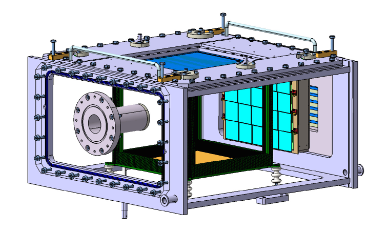
\includegraphics[scale=0.55]{actar.png}
        \caption{ACTAR TPC}
        \label{Fig:2.2.01-actar}
    \end{subfigure}
    \begin{subfigure}[b]{0.45\linewidth} \centering
        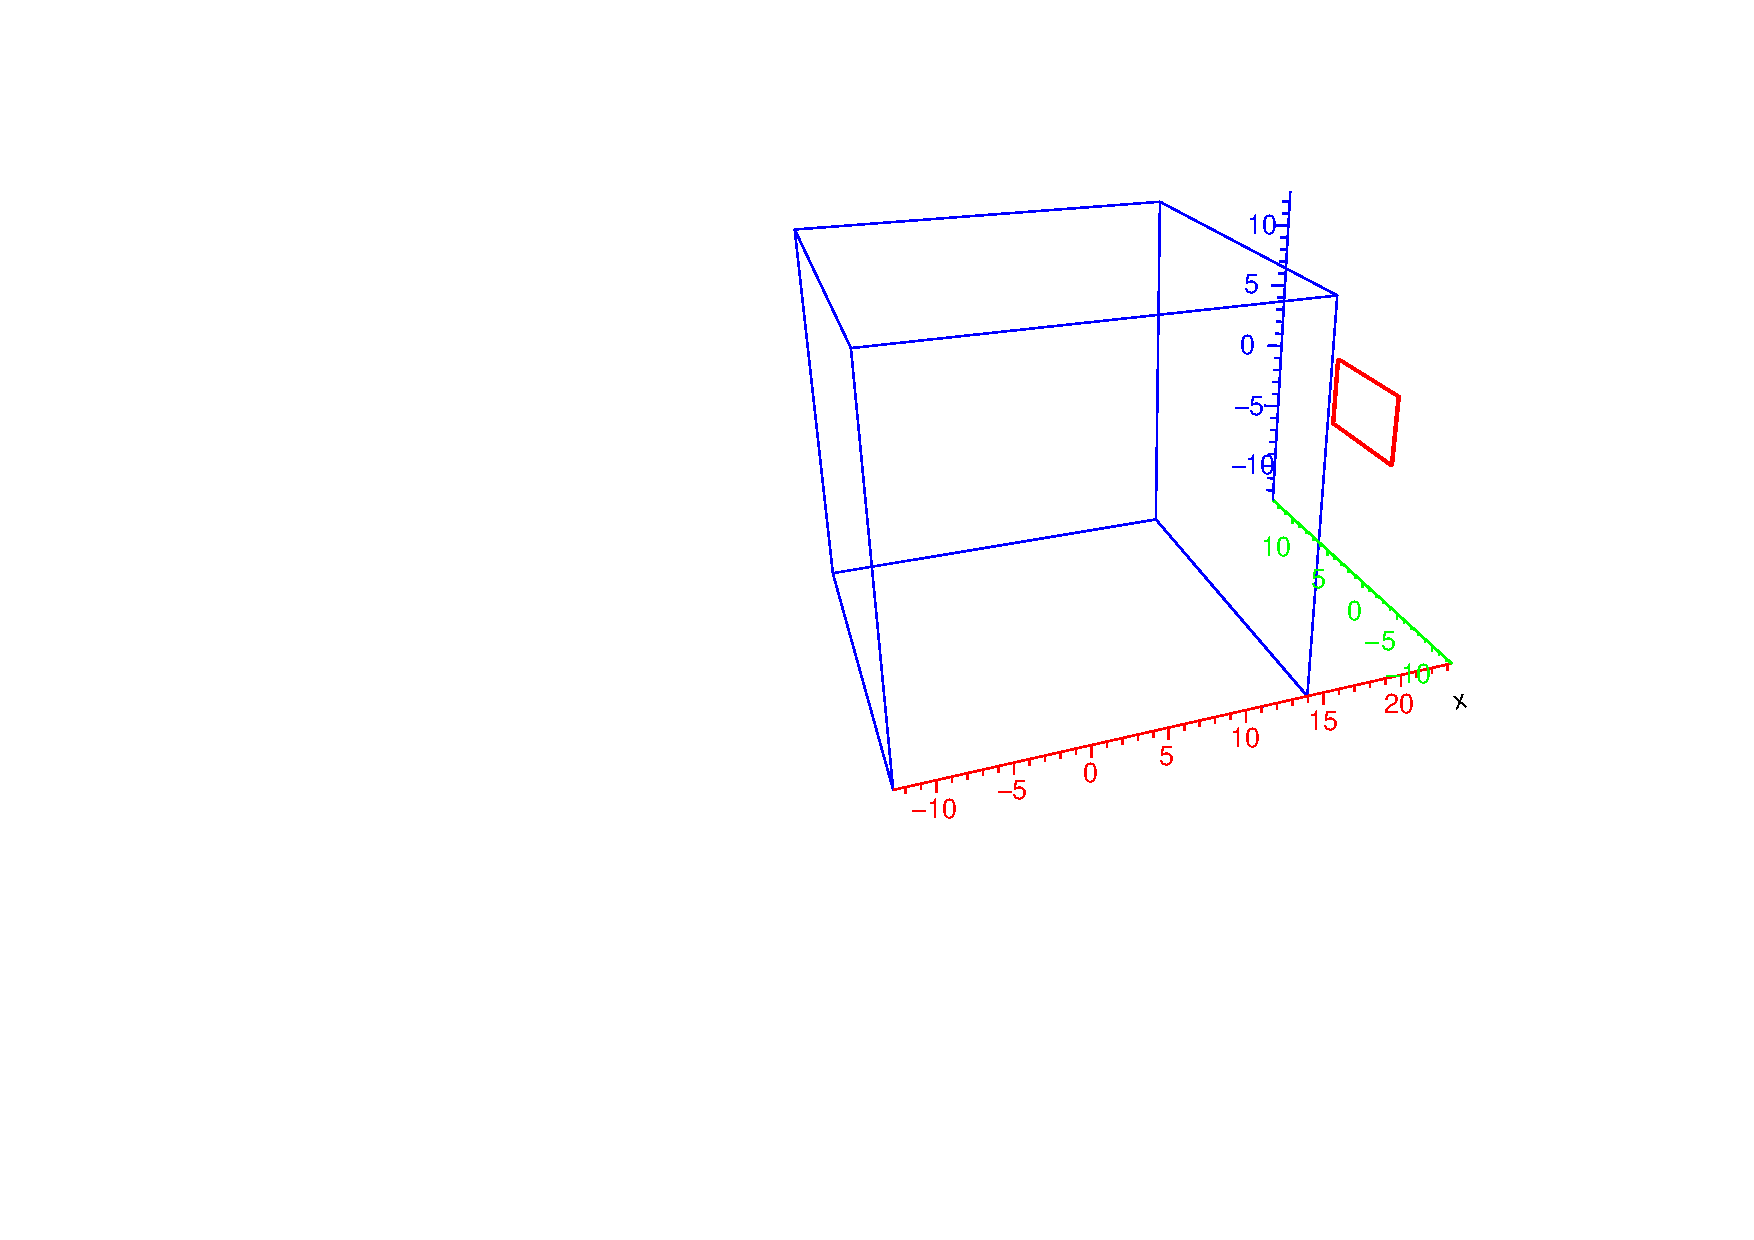
\includegraphics[scale=0.4]{geo.pdf}
        \caption{geometría implementada}
        \label{Fig:2.2.01-geometria}
    \end{subfigure}
    %\caption{Sistemas de referencia para las diferentes partículas}
\end{figure}
    
La función del ACTAR TPC es doble. Por un lado dentro de la caja, donde se encuentra contenido el gas, habrá un campo eléctrico (región que llamamos {\it ACTAR} o {\it TPC}) que nos permitirá medir el movimiento de los átomos a través del gas, ya que  el movimiento de estos ionizará el gas, que debido a la acción campo eléctrico, hará que los electrones se muevan  hacia unos detectores que actuarán como una suerte de condensadores (los detectores se encuentran en la región naranja dentro de la caja negra de la figura \ref{Fig:2.2.01-actar}). Conociedo entonces el recorrido y la velocidad de deriva podremos realizar una construcción tridimensional (siendo una de las dimensiones la temporal). Lógicamente exisitirá una región entre el ACTAR TPC, y los detectores de silicio (presentados a continuación) donde no existirá campo eléctrico, necesaria para poder evitar las interacciones entre el campo eléctrico del pad (3000 V) y la diferencia de potencial de los detectores de silicio (150V), ya que de otro modo se introduciría una fuente de incertidumbre a mayores. En concreto lo que pasaría es que las trazas del campo eléctrico se curvarían, dejando de ser líneas rectas. Una distancia suficiente entre estos sería de 3-5cm, pero como el detector real tiene, además, detectores de las partículas ligeras (en nuestro caso tritio), esta distancia es ampliada hasta unos 15 cm (aproximadamente).  \\

Por otro lado tendremos detectores de Silicio ubicados al final de la caja (cuadrados celestes de la figura \ref{sub@Fig:2.2.01-actar}) que, como veremos, nos permitirá obtener las energías y ángulos de las partículas emitidas tras la colisión. Cabe destacar que el grosor de estos detectores también es muy importante, ya que como vamos a ver, lo que nosotros medimos en el laboratorio es la energía que pierden nuestros átomos en los detectores de silicio. Unos detectores delgados harán que ciertas partículas no se paren, por lo que obtendremos para diferentes ángulos mismos valores de la energía (ya que este tendrá un ``máximo detectable''). A la energía para la cual la partícula se deja de parar la llamamos {\it punchtrough}. Un tamaño de 1.5 mm será más que suficiente para la partícula pesada, ya que la energía máxima de las partículas es de 90 MeV mientras que la de punchtrough (para 1.5 mm) es de 125 MeV.  


\subsection{Trabajo Realizado}

\subsubsection{Cálculo de la cinemática}

La primera tarea realizada fue calcular la cinemática de las partículas. La mejor aproximación que se puede hacer de la reacción se hace dentro de la relatividad especial, debido a las altas energías y la baja masa de las partículas. De manera particular nosotros asumimos que las partículas emitidas no están excitadas (energía de excitación nula). \\

Resolver la cinemática de la colisión consiste en calcular las energías de las diferentes partículas . El sistema de referencia de más interés es el nuestro, que llamamos laboratorio (figura \ref{Fig:2.3.01-Lab}), y es aquel en el que la partícula del litio 11 incide con una energía $T_{beam}$ sobre la partícula de deuterio que suponemos quieta. El otro sistema de referencia de interés es el sistema centro de masas (figura \ref{Fig:2.3.01-CM}). \\

Tras un cálculo que no se incluye aquí pode tema de espacio, pudimos obtener la ecuación de la energía cinética de las partículas y su ángulo de salida (respecto el eje de incidencia) en el sistema laboratorio a partir de dos parámetros: el ángulo de salida de la partícula en el sistema de centro de masas, y de $T_{beam}$. Dado que este último es un valor conocido, podríamos obtener $\theta_4$ y $\theta_3$ a partir de $T_3$ y $T_4$.   \\

\begin{figure}[h!] \centering
\begin{subfigure}[b]{0.45\linewidth} \centering
    \begin{tikzpicture}[thick,scale=0.8] 
    \node (1) at (-3,0+1.24) {};
    \node (2) at (0,0+1.24) {$m_2$};
    \node (3) at (3,1+1.24) {$m_3$};
    \node (4) at (3,-1+1.24) {$m_4$};
    \node (m1) at (-1.5,0.5+1.24) {$m_1$};
    \node (h) at (0.0,0.0-2*0.5) {};
    \draw[arrows={->},ultra thick] (1.east)--(2.west);
    \draw[arrows={->},ultra thick] (2.east)--(3.west);
    \draw[arrows={->},ultra thick] (2.east)--(4.west);
    \end{tikzpicture}
    \caption{Sistema Laboratorio}
    \label{Fig:2.3.01-Lab}
\end{subfigure}
\begin{subfigure}[b]{0.45\linewidth} \centering
    \begin{tikzpicture}[thick,scale=0.8] 
    \node (1) at (-3.5,0) {};
    \node (2) at (3.5,0) {};
    \node (3) at (1.8,2.8*0.8) {};
    \node (4) at (-1.8,-2.8*0.8) {};
    \draw[arrows={->},ultra thick] (1.east)--(-0.1,0)  ;
    \draw[arrows={->},ultra thick] (2.west)--(0.1,0)  ;
    \draw[arrows={->},ultra thick] (0.1,0.1)--(3.south west)  ;
    \draw[arrows={->},ultra thick] (-0.1,-0.1)--(4.north east)  ;
        
    \node (m1) at (-1.75,0.3) {$m_1$};
    \node (m2) at (1.75,0.3) {$m_2$};
    \node (m3) at (2.3,1.8) {$m_3$};
    \node (m4) at (-2.1,-1.8) {$m_4$};
    \end{tikzpicture}
    \caption{Sistema Centro de Masas}
    \label{Fig:2.3.01-CM}
\end{subfigure}
%\caption{Sistemas de referencia para las diferentes partículas}
\end{figure}

\subsubsection{Introducción a C++}

Nuestro segundo paso fue aprender la sintáxis básica de C++ y ROOT. Para esto realizamos algunos programas básicos, que consistían en realizar histogramas y algunas gráficas; así como la definición de variables y de funciones. Otra de las partes mas importantes fue la implementación de la geometría, esto es, la disposición del detector. La figura \ref{Fig:2.2.01-geometria} es una representación gráfica de lo que tenemos en cuenta de la geomertría: dimensiones de cada lado (25.6 cm) así como distancia entre ACTAR TPC y detector de silicio (9 cm), así como el número de detectores de silicio (en nuestro caso 1, en el centro), la dimensión de estos (8 cm x 5 cm) y su grosor (1.5 cm).

\subsubsection{Implementación de la simulación} \label{Subsubsec:implementacion}
Una vez acabamos de introduccirnos a C++ empezamos a implementar la simulación. Lo primero que hicimos fue comprobar si los cálculos  de la cinemática realizados eran correctos. Para la implemetnación de estas ecuaciones se crearon diferentes clases, modularizando el programa principal, de tal modo que matuvimos bien organizadas las diferentes funciones. Dado que no conocemos el ángulo con el que van a salir las partículas, ya que este es un parámetro libre, usamos una clase para todo el intervalo de $\theta_{cm}$ (entre 0 y 180 grados). En la siguiente imagen podemos ver la cinemática del tritio (\ref{sub@Fig:2.2.01-hidrogeno}) y la del litio (\ref{sub@Fig:2.2.01-litio}), que es la de interés.   \\

\begin{figure}[h!] \centering
    \begin{subfigure}[b]{0.45\linewidth} \centering
        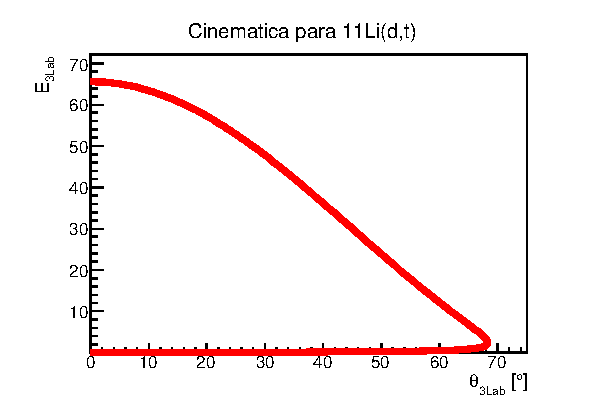
\includegraphics[scale=0.8]{CinematicaH.eps}
        \caption{cinemática tritio.}
        \label{Fig:2.2.01-hidrogeno}
    \end{subfigure}
    \begin{subfigure}[b]{0.45\linewidth} \centering
        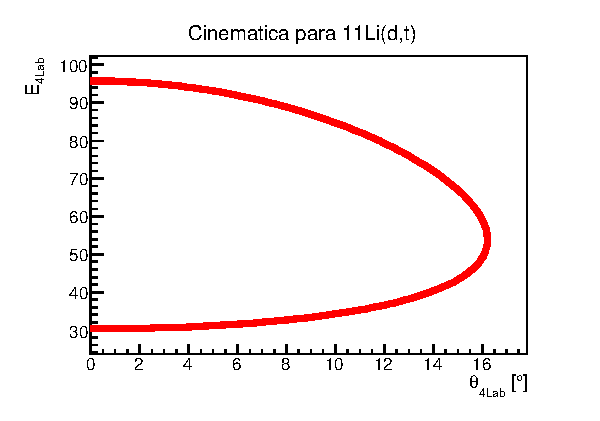
\includegraphics[scale=0.8]{Cinematica11Li.eps}
        \caption{cinemática litio 10 (gráfica de interés).}
        \label{Fig:2.2.01-litio}
    \end{subfigure}
    %\caption{Sistemas de referencia para las diferentes partículas}
\end{figure}
    

Una vez comprobamos que la cinemática se calculó correctamente, podemos comenzar a construir la simulación. Esto implica implementar a la colisión los diferentes factores a tener en cuenta. 


\begin{enumerate}

    \item  Primero tenemos que obtener cual es el vértice de la reacción (punto donde se produce la reacción), el cual tendremos que obtener mediante una variable aleatorio. 
    
    \item También tendremos que introducir el ángulo de salida, para el cual creamos una variable aleatoria para el ángulo $\theta_{CM}$. Un factor que no hemos tenido en cuenta ha sido el de la {\it sección eficaz diferencial}, ya que hemos hecho una simplificación al asumir que $\theta_{CM}$ esta uniformemente distribuido cuando este en realidad vendrá pesado por la {\it sección eficaz diferencial}, que no está incluido. De hecho es en este observable en el que está contenida la información física de la estructura interna del núcleo. 
    
    \item Lo tercero que tenemos que hacer es ver si el litio 10 que se emite en el vértice llega al detector de silicio. Para saber si es detectado o no, basta con extender la trayectoria de la partícula (suponiendo que se mueve en una línea recta) y ver si llega al detector. Para esto hay que tener en cuenta las dimensiones del detector.     

    \item También habrá que tener en cuenta las pérdidas de energía, ya que si la partícula llega con energía cero no podrá ser detectada. Para esto tenemos que implementar la ecuación de Bethe-Bloch para la partícula incidente y para la partícula pesada dentro del detector de silicio. Siempre que la partícula llegue al detector con energía cero la partícula no podrá ser detectada, por lo que tendremos que incluir este factor. En la imagen \ref{Fig:energia_perdida} podemos ver la pérdida de energía de una partícula en función de la distancia, para el cual usamos el programa SRIM. 
    
    \begin{figure}[h!] \centering
        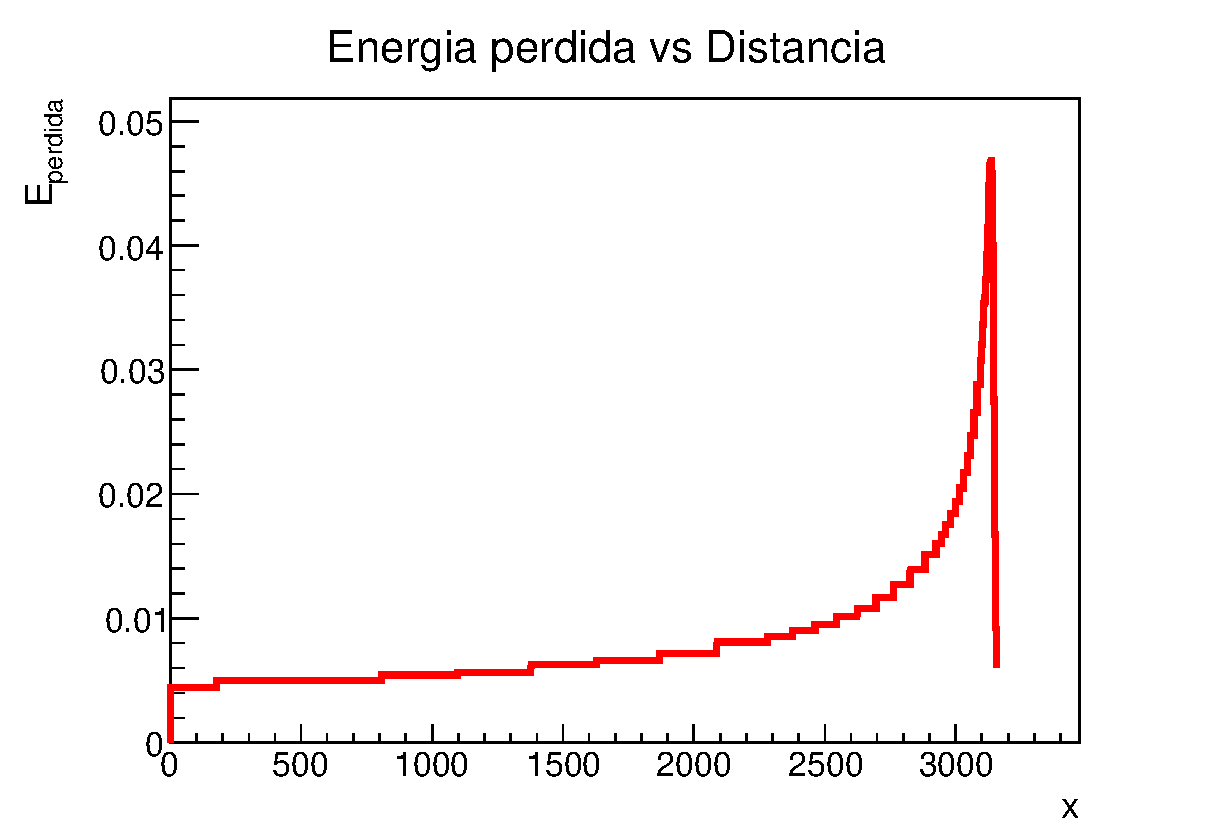
\includegraphics[scale=0.7]{srim.eps}
        \caption{energía perdida frente a la distancia según la ecuación Bethe-Bloch.}
        \label{Fig:energia_perdida}
    \end{figure}

\end{enumerate}

Una vez acabamos con esto ya tendremos la simulación, en su versión más básica. Como esta es una simulación del experimento real, nosotros tendremos que volver a obtener, con los datos finales y medibles (energía périda en el silicio $\Delta E$, ángulo de la partícula 4) los datos que queremos obtener (energía al salir de la colisión de la partícula 4, ángulo de la partícula 4). Esto implicará una {\it reconstrucción} de la cinemática a partir de estos datos. En ese caso tendremos que añadir algún tipo de incertidumbre en este proceso de pérdida de energía dentro del silicio. Estas vendrán dadas por dos factores. \\


El primero de estos es considerar que la perdída de energía es un proceso estadístico, por lo que dos partículas con la misma energía inicial no van a llegar con la misma energía al detector de silicio. El segundo es considerar la resolución de nuestros dectectores de energía, ya que energías muy próximas no podrán ser distinguibles. 

\begin{itemize}
    \item Para incluir el fenómeno estadístico de la pérdida de energía tendremos que tener en cuenta la energía inicial y la distancia que va a recorrer por el medio. Para introducir la energía pérdida de un modo estadístico lo que haremos será lo siguiente: primero evaluaremos el rango de la partícula con la energía inicial ($R_L$) (esto es, la distancia antes de que se pare la partícula) con su respectiva incertidumbre ($u(R_L$)). Dado que la distancia es la traza, esto es, la distancia del vértice al silicio (que llamaremos $d$), la cual es conocida, podremos evaluar cual es la distancia recorrida con una simple resta ($R_{left}=R_L-d$). Luego podremos evaluar $u(R_{left})$ con la misma ecuación, de tal modo que podamos despejar $u(d)$. Con la incertidumbre y con $d$ crearemos un nuevo valor $d'$ como una gaussiana $\mu=d$ y $\sigma=u(d)$. Luego calcularemos $R'_{left}=R_{L}-d'$, pudiendo recuperar la nueva energía con la que sale del detector usando (conocido el rango y el medio, podremos calcular la energía inicial). Así luego solo tendremos que realizar la diferencia entre la energía entrante y la energía de salida para obtener la energía perdida ($\Delta E$) en el gas. 
    
    \item La resolución debida a medir con detectores de silicio usando semicontuctores p ha sido estudiado ampliamente por la física electrónica, por lo que simplemente usaremos datos ya tabulados para incluir. Sabiendo que la $\sigma$ era de 50 keV para una perdida de energía de 5.5 MeV (medida con una fuente triple alfa en otros experimentos), usamos la siguiente fórmula para extrapolar la energía, sabiendo que la resolución depende de la raíz de la energía $E$: 
    
    \begin{equation}
        \sigma = \frac{0.0213 \  \text{MeV}}{2.35} \sqrt{E}
    \end{equation}
    podremos obtener una $\Delta E$ aplicando una gaussiana con dicha media y esa $\sigma$ a través de la librería TRandom de ROOT. 

\end{itemize}




Una vez tenemos todo esto ya tenemos una simulación del experimento mucho más realista, donde podamos obtener los resultados tal y como los mediríamos en el laboratorio, y compararlos con los que obtenemos en la simulación. Idealmente ambos deberán coincidir, aunque como veremos, debido a los factores anteriores (resolución, pérdidas estadísticas) no se verificará. Como podemos ver en las figuras siguientes, para dos distancias diferentes obtenemos un patrón similar: las partículas más detectadas son aquellas de ángulos bajos, mientras que existe una región de dispersión mucho má grande para las energías. También se puede verificar que para las distancias de 17 cm las partículas detectadas son menos que las partículas detectadas para 5 cm (para los ángulos más grandes principalmente). 

\begin{figure}[h!] \centering
    \begin{subfigure}[b]{0.45\linewidth} \centering
        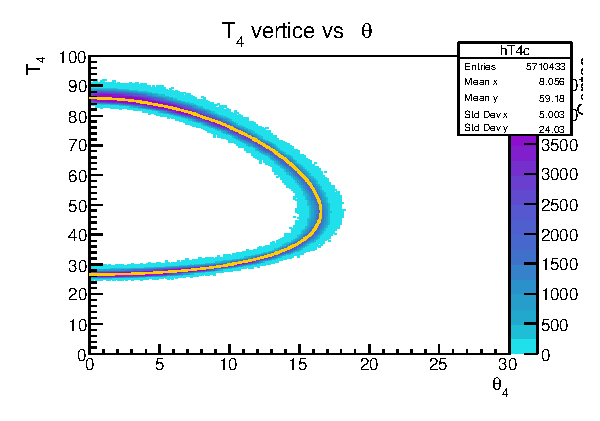
\includegraphics[scale=0.8]{5_measured_kin.eps}
        \caption{particulas reconstruidas para 5cm.}
        \label{Fig:2.3.01-measured-5}
    \end{subfigure}
    \begin{subfigure}[b]{0.45\linewidth} \centering
        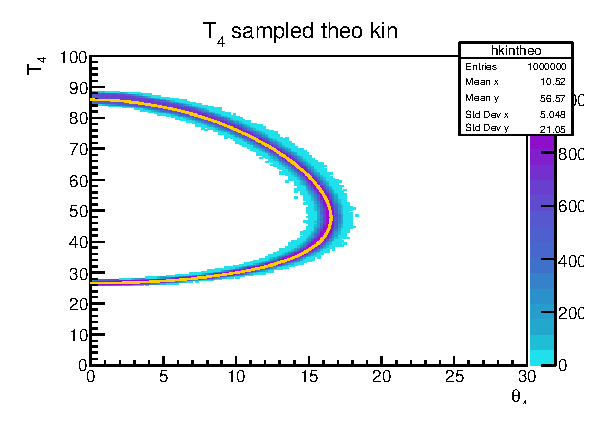
\includegraphics[scale=0.8]{5_simulation_kin.eps}
        \caption{particulas realmente emitidas para 5cm.}
        \label{Fig:2.3.01-theo-5}
    \end{subfigure}
    \caption{cinemáticas medidas vs reales emitidas para una distancia de 5 cm.}
\end{figure}
    
\begin{figure}[h!] \centering
    \begin{subfigure}[b]{0.45\linewidth} \centering
        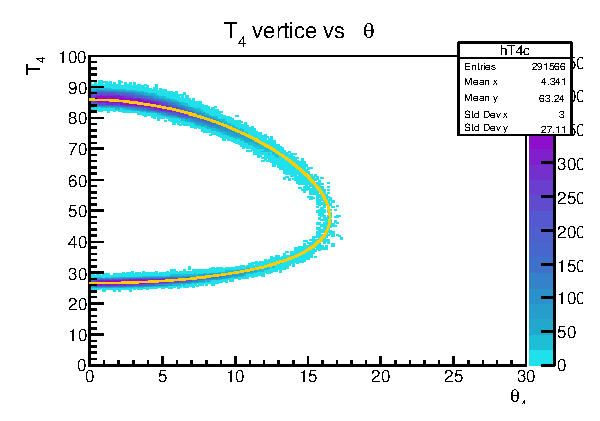
\includegraphics[scale=0.8]{17_measured_kin.eps}
        \caption{particulas reconstruidas para 17cm.}
        \label{Fig:2.3.02-measured-17}
    \end{subfigure}
    \begin{subfigure}[b]{0.45\linewidth} \centering
        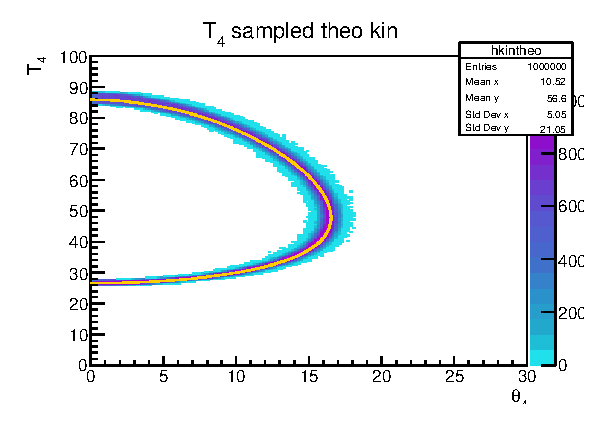
\includegraphics[scale=0.8]{17_simulation_kin.eps}
        \caption{particulas realmente emitidas para 17 cm.}
        \label{Fig:2.3.02-theo-17}
    \end{subfigure}
    \caption{cinemáticas medidas vs reales emitidas para una distancia de 17 cm.}
\end{figure}
    



\subsection{Resultados}

Como ya hemos dicho nos interesa reducir la incertidumbre de la parte angular lo máximo posible. La incertidumbre del factor ángulo, que es lo que estamos tratando de estudiar, está relacionada con la $\sigma$ de la gaussiana que se forma para una determinada energía, por lo que en función de la energía de la partícula 4 tendremos una $\sigma$ (y una $s(\sigma)$). Sin embargo no todas los ángulos obtenidos para un rango de energías determinado se comportan de manera gaussiana, solo aquellas que se encuentran en la parte central, para ángulos relativamente altos, tal y como se señala en la imagen \ref{Fig:2.4-region_interes}. 

\begin{figure}[h!] 
    \begin{tikzpicture}
        \node[anchor=south west,inner sep=0] (image) at (0,0) { 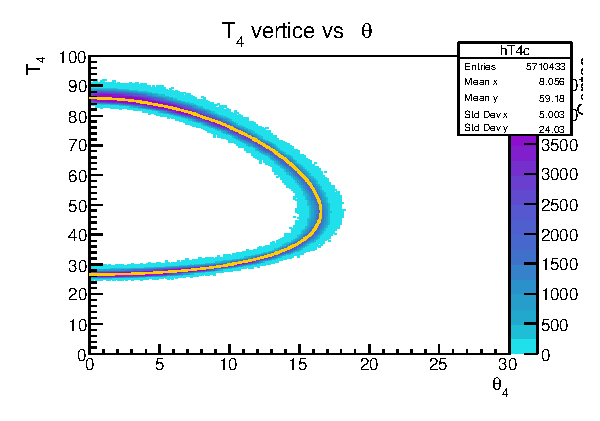
\includegraphics[scale=1]{5_measured_kin.eps}};
        
        \node (1) at (6.5,4.5) {};
        \node (2) at (6.5,3.5) {};
        \node (3) at (5.2,3.5) {};
        \node (4) at (5.2,4.5) {};

        \node (f0i) at (9.6,3.5) {};
        \node (f0f) at (11.5,3.5) {};

    \draw[ultra thick]  (5.8, 2.8)-- (4.4,2.8)  -- (4.4,3.8) -- (5.8,3.8) -- (5.8,2.8) ;
    \
    \draw[arrows={->},ultra thick] (f0i)--(f0f); 

    \node[anchor=south west,inner sep=0] (image) at (11.3,-0.6) { 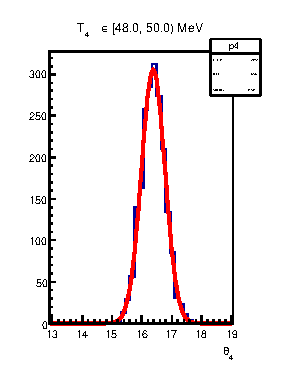
\includegraphics[scale=1.3]{15_fit.eps}};
        

    \end{tikzpicture}
    \caption{región de interés, distancia 15 cm.}
    \label{Fig:2.4-region_interes}
\end{figure}


Lo que hicimos nosotros para calcular la $\sigma$ para cada una de las distancias fue crear histogramas con los ángulos para un intervalo de energía de 2 MeV, entre las energías 40 y 56, de tal modo que obtenemos una $\sigma$ para cada uno de los intervalos de energía y las distancias, lo cual hemos representado en la imagen \ref{Fig:2.4-sigma} (la distancia de 50 cm no fue representada por que alteraba la gráfica). Como se puede ver en dicha imagen, en los intervalos mas extremos la $\sigma$ y $s(\sigma)$ comienza aumentar, ya que las regiones comienzan a tener comportamientos menos gaussianos, como es de esperar.  \\

También realizamos un estudio de la eficiencia, la cual ROOT nos permite calcular de manera sencilla a partir del número de partículas emitidas para un ángulo y el número de partículas {\it realmente} medidas. Como podemos ver en la imagen \ref{Fig:2.4-Efficiencia}, la eficiencia cae abruptamente con la distancia, mientras que la $\sigma$ tiene un comportamiento constante (salvo por la  $s(\sigma)$ para la distancia de 17 cm). \\

Como podemos ver el valor de $\sigma$ (0.4$^\circ$) si lo convertimos a FWHM (0.94$^\circ$) obtenemos un valor aproximadamente de 1$^\circ$, que fue el valor que implementamos en la creación de la variable angular (paso 2 de la implementación, subapartado \ref{Subsubsec:implementacion}), de lo cual se deduce  que la las contribuciones implementadas (straggling, resolución) no afectan mucho a la $\sigma$. 


%Tes que comentar que  a eficiencia claramente decrece coa distancia e que a  incerteza angular fica aproximadamente constante para todas as distancias. O seu valor de 0.4 deg, se o convertes a FWHM (* 2.35) ves que coincide co straggling angular que implementaches na variable angular aquí; é dicir, as contribucións do straggling en enerxía e resolución non afectan moito. O valor de 1 deg FWHM que implementaches foi derivado da análise de experimentos pasados en configuracións similares do detector.


\begin{figure}[h!] \centering
    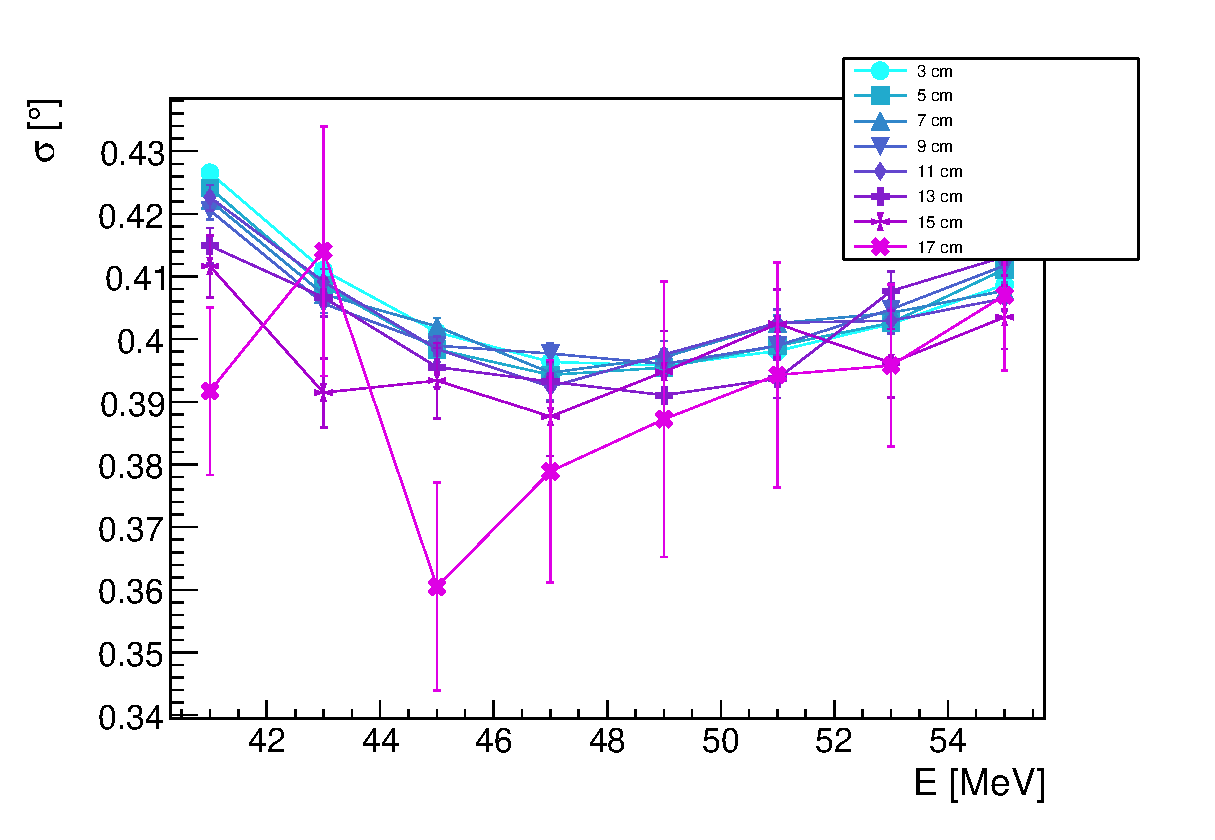
\includegraphics[scale=0.8]{sigma.eps}
    \caption{valores de $\sigma$ en función de la distancia y para cada intervalo de energías.}
    \label{Fig:2.4-sigma}
\end{figure}

\begin{figure}[h!] \centering
    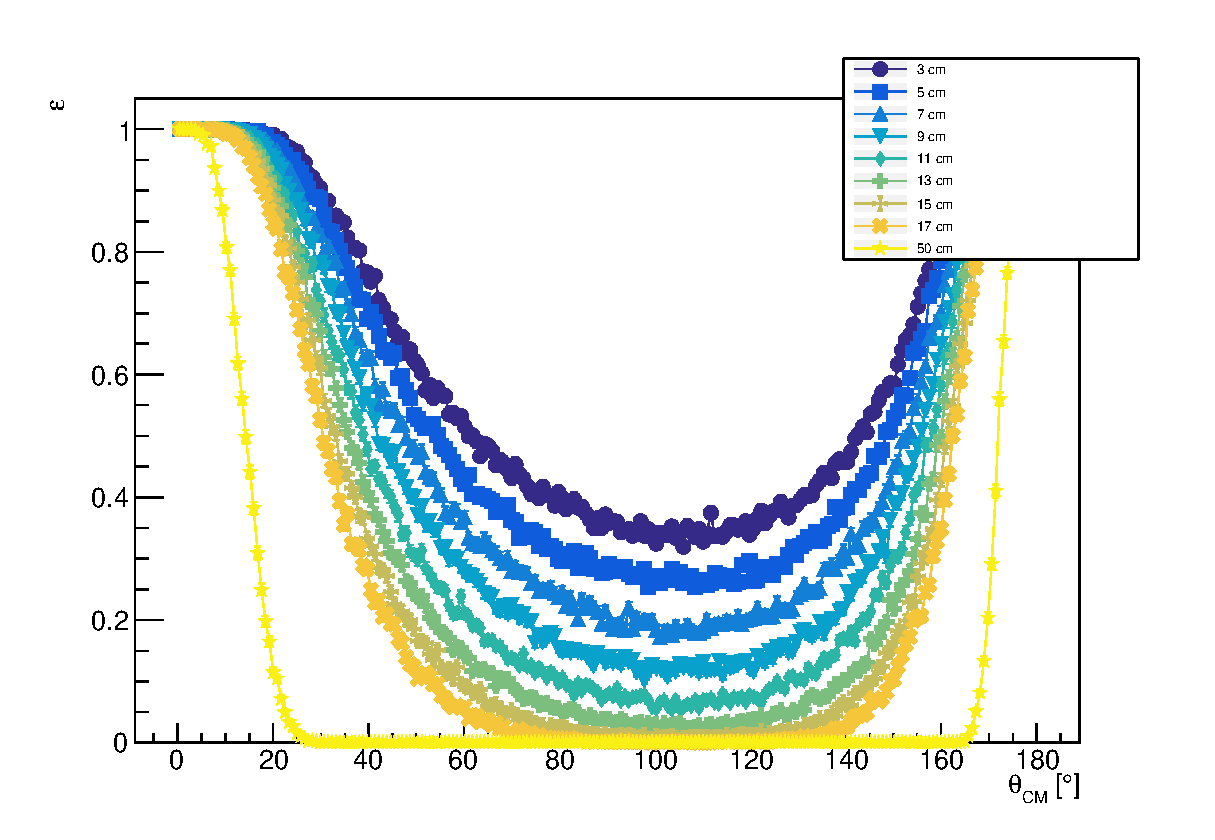
\includegraphics[scale=0.8]{Eff.eps}
    \caption{eficiencia en función de la distancia.}
    \label{Fig:2.4-Efficiencia}
\end{figure}


\section{Conexión con el grado en física}

Las asignatuas más relacionadas con estas prácticas son {\it Fisica nuclear y de partículas} y {\it Técnicas Experimentales IV}, ambas del 4º curso del grado. La relación que tiene esta práctica con la primera asignatura está, esencialmente, en la parte de las reacciones nucleares y su cinemática, una parte fundamental de dicha asginatura, la cual hemos podido implementar en un problema a la vanguardia científica, demostrando su validez. La relación con la segunda asignatura es clara, ya que hemos necesitado implementar histogramas y ciertas herramientas informáticas fundamentales en la asignatuas, así como conceptos relacionados con la física experimental (detectores de Silicio, estadística derivada de la colisión de partículas...) que también se ven en la misma. 


\section{Valoración personal}

Mi valoración tras la realización de estas prácticas es muy positiva, ya que he podido conocer como funciona por dentro un grupo de investigación experimental, pudiendo ver de primera mano cual es el poder de las herramientas informáticas y de simulación que existen hoy en día, para poder predecir el experimento e incluso mejorarlo sin necesidad de experimentar. Además de esto poder aprender un nuevo lenguaje de programación, tan útil en estos días como es C++, así como la herramienta ROOT para poder evaluar y rellenar histogramas, me parece fundamental para un físico. \\

Más allá de los conocimientos adquiridos, que es el motivo principal por lo que solicité estas prácticas, y los cuales, he de decir, han superado mis expectativas, me quedo con la experiencia de realizar un proyecto muy divertido, interesante y el cual me ha enseñado que la física nuclear e incluso la física experimental es mucho más de lo que se valora en el ámbito académico.


\end{document}



